\documentclass[conference]{IEEEtran}
\IEEEoverridecommandlockouts
% The preceding line is only needed to identify funding in the first footnote. If that is unneeded, please comment it out.
\usepackage{cite}
\usepackage{amsmath,amssymb,amsfonts}
\usepackage{algorithmic}
\usepackage{graphicx}
\usepackage{textcomp}
\usepackage{xcolor}
\def\BibTeX{{\rm B\kern-.05em{\sc i\kern-.025em b}\kern-.08em
    T\kern-.1667em\lower.7ex\hbox{E}\kern-.125emX}}
\begin{document}

\title{NAO robot that imitates human movements using Mediapipe\\

}

\author{\IEEEauthorblockN{Costilla Caballero, Salvador}
\IEEEauthorblockA{\textit{Applied Robotics } \\
\textit{Hof University of Applied Science}\\
CDMX, Mexico \\
salvadorcoscab@gmail.com}
}

\maketitle

\begin{abstract}
In this project, we programmed a NAO robot from Aldebaran to mimic human movements captured by a webcam using Mediapipe. While this type of human imitation has been done before, we aimed to approach it differently. Unlike most other projects utilizing multiple cameras or depth sensors like the LIDAR sensor, our focus was on a novel methodology.
The project is still in progress, with the robot currently capable of moving its arms, albeit not with high precision. Nonetheless, we see this as a promising starting point for future developments in computer vision and robotics.
\end{abstract}

\begin{IEEEkeywords}
NAO, Mediapipe, Human imitation, aldebaran, robotics
\end{IEEEkeywords}
% State of the art
\section{State of the art}
In this section, we will explore various methods for controlling the movement of a NAO robot using the Mediapipe Framework, as well as discuss related work involving human imitation with the NAO robot.

According to the NAO robot documentation \cite{b1}, there are two primary methods for posing the NAO robot: using joint angles and employing inverse kinematics. While other methods exist for walking or performing predefined poses, these two are fundamental to our project's scope.

Regardless of whether inverse kinematics is employed, there are two main ways to control the effectors to achieve a pose:
\begin{itemize}
    \item Animation methods, which operate within fixed time frames and involve blocking functions.
    \item Reactive methods, suitable for real-time control with non-blocking functions.
\end{itemize}

Within the \textit{ALMotionProxy} module, numerous functions pertain to joint movement. Some notable animation methods include:
\begin{itemize}
    \item \textit{ALMotionProxy.angleInterpolation}, enabling movement from one specific position to another within a specified time.
    \item \textit{ALMotionProxy.angleInterpolationWithSpeed}, facilitating movement between specific positions within defined time and speed parameters.
\end{itemize}
An essential method is:
\begin{itemize}
\item \textit{ALMotionProxy.setAngles}, enabling the manipulation of single joint angles or sets of joint angles on the robot.
\end{itemize}

Furthermore, the robot's control extends to inverse kinematics. Here, classical IK solvers and generalized IK solvers (Whole Body control) are employed. Some pertinent animation and reactive methods related to inverse kinematics include:
\begin{itemize}
    \item \textit{ALMotionProxy.positionInterpolation}, facilitating movement between specific positions within a specified time frame.
    \item \textit{ALMotionProxy.setPosition}, enabling precise positioning of the robot in 3D space.
\end{itemize}

BlazePose \cite{b2} is an architecture for single-person 3D pose detection based on convolutional neural networks. It is integrated into the Mediapipe framework, enabling the detection of poses from videos or images. The model is capable of detecting 33 landmarks (see Figure \ref{fig:landmarksMP}), which can be interpreted as points in a 3D space.

\begin{figure}[htbp]
\centerline{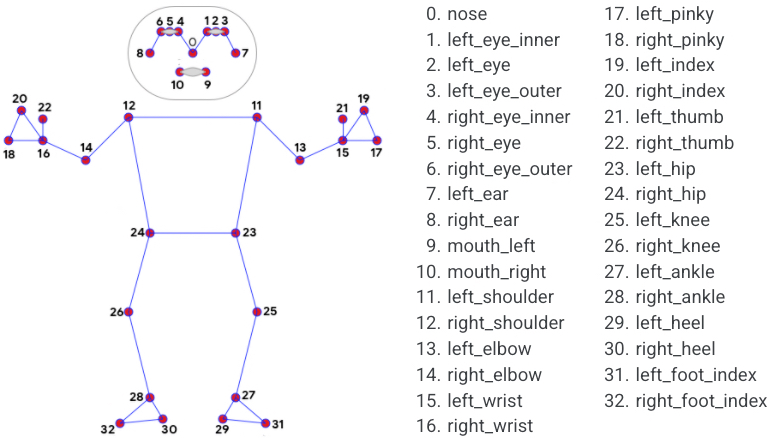
\includegraphics[width=0.48\textwidth]{images/landmarksMP.jpeg}}
\caption{Landmarks from the Mediapipe library.}
\label{fig:landmarksMP}
\end{figure}

The Landmarker offers various configuration options, including:

\begin{itemize}
\item \textit{model\_complexity}, This parameter allows selection among three different models - lite, full, and heavy. Depending on the chosen model, both accuracy and speed can vary.
\item \textit{min\_detection\_confidence}, It enables setting the minimum confidence level required for detecting a pose.
\item \textit{min\_tracking\_confidence}, This parameter allows setting the minimum confidence level required for tracking a pose.
\end{itemize}

In a thesis titled "Mimetización de movimiento por robot antropomorfo basado en imágenes de sensor de profundidad" \cite{b3}, the authors utilize the NAO robot to mimic human movements using a Kinect sensor. They adopt a client-server approach to transmit data from the Kinect sensor to the robot via the NAOqi API. In the client-side implementation, they employ the \textit{pykinect2} library to retrieve data from the Kinect sensor, which consists of 25 landmarks representing the human body. This data is then relayed to the server-side using the \textit{socket} library. On the server-side, the angles between the joints are computed and transmitted to the robot using the \textit{ALMotionProxy.AngleInterpolation} method.
% intrduccion: poner en contexto al lector sobre el tema
% Se describe el orden de los estudios
% revisar el proyecto del kinect 
% revisar formas de conectar multiples versiones de python
% revisar mediapipe pose estimation
% revisar NAOqi API
% revisar robot NAO
% investigaciones, proyectos, papers, etc.: describir nombres de las referenciadas
% conclusiones de la investigacion


\section{Approach}

\subsection{Objectives}

During this project we had some objectives which were:
\begin{itemize}
\item Solve the computer vision part, that in this case was done with Mediapipe.
\item Make the robot move using the NAOqi API.

\end{itemize}
The problems were that, in order to work with the NAOqi API, we had to download and setup the SDK which is written (by the moment of this project) in Python 2.7 and the Mediapipe is only availble in Python 3.7 or higher. That is why we had to add as an objective to make the two libraries work together.


% Methodology
\subsection{Methodology}
The methodology that we used to solve the objectives above was to first divide the problem into modules and try to solve them separately, and then join them together and solve the problems that arose from the connection between the two modules.
The main two modules were the computer vision and the robot movement.


\subsection{Computer vision}
% Begin with the computer vision part and the NAOqi API part
In the beginning, the computer vision part was done very easily, because Mediapipe has a lot of usage examples and good documentation, such as the video "AI Pose Estimation with Python and MediaPipe"\cite{b4}, that helped us a lot on getting the landmarks and calculate some angles. On the other hand working with the NAO robot was a much more difficult, because we did not know how to start.
\\
For the computer vision part we used the opencv library to get images from both camera and videos and then we used the Mediapipe library to get the poses from the images.
We used also the opencv library to plot the landmarks that the Mediapipe library detected, so  we could see how the landmarks were being detected. This landmarks conformed an object with 33 points, which represents landmarks of the human body. (See figure \ref{fig:landmarksMP})


\subsection{Robot movement}

Then we started working with the robot movement part, to do this we used the NAOqi API. We realized, after reading the NAOqi documentation that there is two ways to control the robot for doing poses. The first one was using angles and the second one was using inverse kinematics. 
We decided to use the first one because we thought that with the landmarks, obtained with Mediapipe, we could easily get the angles of each join of the robot, and also the project that we found on internet used this approach.
All of this joint-angle approach is written in the \textit{ALMotion} module of the NAOqi API. 
In summary the robot has various joints, and each joint can be moved using a specific angle. These joints work in a similar way as the human body joints, allowing some joints to pitch, roll, and yaw. (See figure \ref{fig:RightArmAngles})

\begin{figure}[htbp]
    \centerline{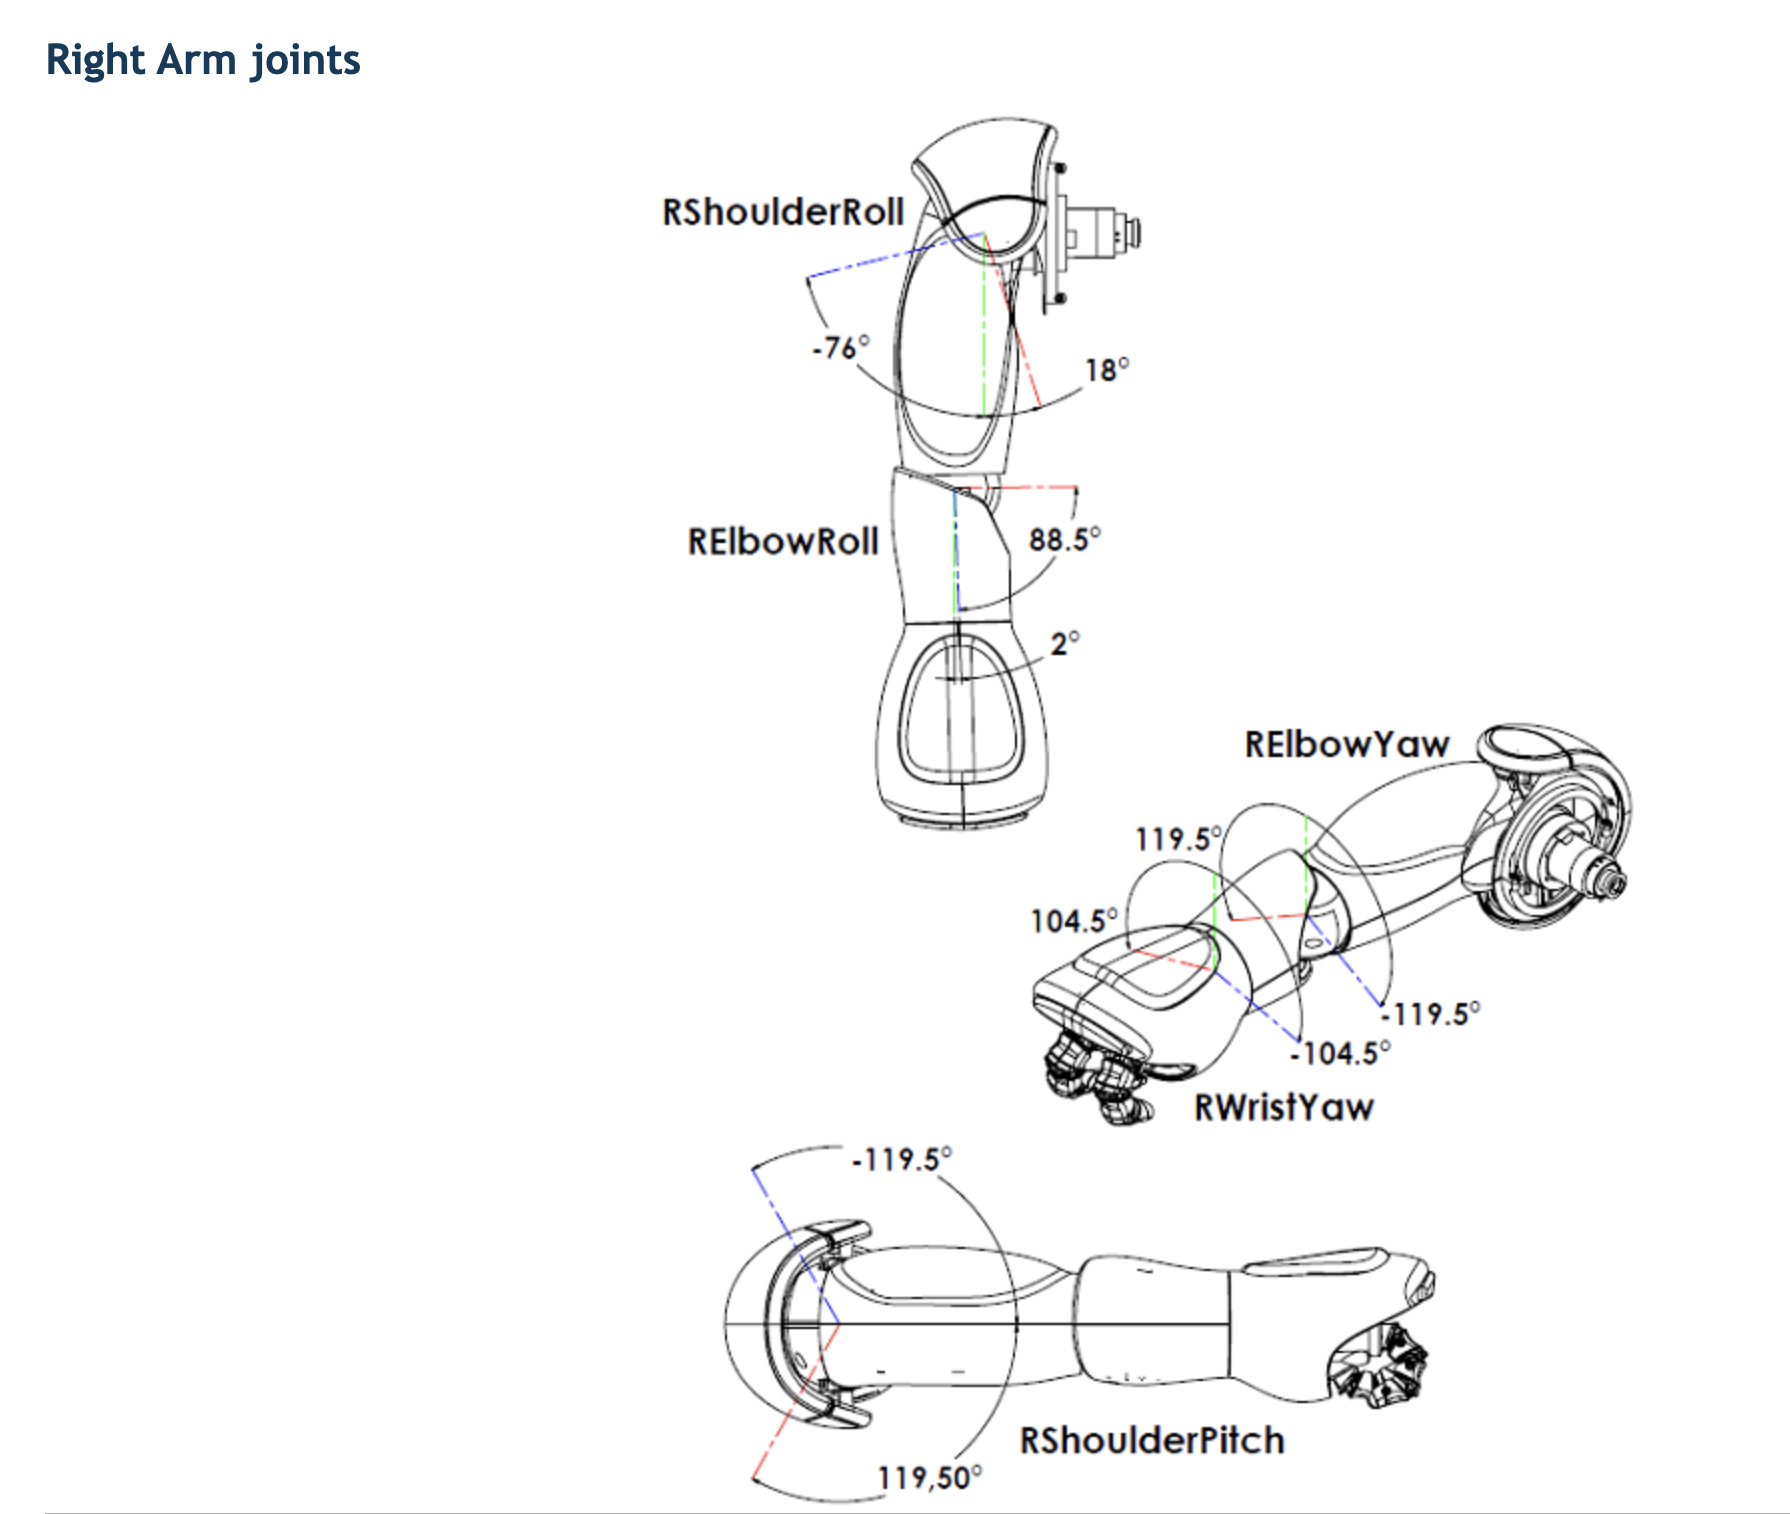
\includegraphics[width=0.5\textwidth]{images/RightArmAngles.jpeg}}
    \caption{Landmarks from the Mediapipe library.}
    \label{fig:RightArmAngles}
    \end{figure}

% connection between the two parts
\subsection{Connection between the Computer vision and the Robot movement}
After doing some testing on both parts, we had to somehow connect them. In order to do the connection between the robot and the computer vision part, we tried with \textit{execnet}, which is a library that allows you to trigger python scripts from another python script, even with different versions of python. But we had some problems sending the data from the computer vision part to the part in which we move the robot, so we decided to try a different approach.

We decided to use sockets to send the data, as we got inspiration from a project that we found with a similiar approach, in which the author used sockets to send the data from a kinect sensor to the robot.
This solved everything, about the connection between the scripts, because it uses the client-server approach, allowing me to use python 3.10 for the computer vision part that is the client and python 2.7 for the Robot movement part that is the server. We just had to do some encoding to send the data. 

% testing the implemented code
\subsection{Testing the implemented code and solving problems}
After changing the code that we found to work with Mediapipe and OpenCV instead of the kinect sensor. We did some testing on the functions that were already implemented in the server side, but they performed very bad, but at least, we saw that the robot moved.

Also the display of the images was very slow since the code had a delay to send the data, in order for the server to process it. We solved this using a thread to get the data from the displayed image and send it to the server with the thread without messing up with the display.
\\
As we said before after changing a lot the parameters and definition of the functions that were implemented before we realized that we was not sending the right data to the robot from the server, so we decided to change the approach and instead of sending the coordenates of the landmarks to the server, we decided to send the angles between them and send them directly to the server. This would help me to see what angles we was sending to the robot by showing them on the displayed image.

After we was able to see the angles that were being sent to the robot, we realized that the angles sent were not very good in the function definition, this is because the kinect sensor and Mediapipe have different coordenate systems, so we had to change the defintion of the functions.
\\
This did not work very well, though the movements were more accurate, the robot was not imitating the movement of the hands perfectly. So we decided to change the function. Instead of using geometry we tried with vectors and the angles between them.

\subsection{Vector approach}
We saw that as we had the landmarks, that represents a point in the space, we could calculate a vector between two points (See equation \ref{eq:vector}), and we could use the angles between the vectors to move the robot (See equation \ref{eq:angle}). But then we realized that we could also calculate the angles between the projection of the vectors (See equation \ref{eq:proy}) in a generated plane from a normal vector (See equations \ref{eq:plano},\ref{eq:p},\ref{eq:p0}). We tried this for one joint, that was the right shoulder pitch. We got the normal vector from the left shoulder to the right shoulder to generate the plane, and then we got the vectors from the right shoulder to the right elbow and from the shoulder to the right hip. We projected these vectors in the generated plane and then we calculated the angles between them. 
% ecuacion para obtener un vector entre dos puntos
\begin{equation}\label{eq:vector}
    \vec{v} = \vec{p_2} - \vec{p_1}
\end{equation}

% ecuacion para el angulo entre dos vectores para los angulos en el plano generado por el vector normal
\begin{equation}\label{eq:angle}
    \cos(\theta) = \frac{\vec{v} \cdot \vec{w}}{\| \vec{v} \| \| \vec{w} \|}
\end{equation}
% ecuacion de la proyeccion de un vector en el plano esto nos da un vector en el plano generado por el vector normal
\begin{equation}\label{eq:proy}
    proy_H \vec{v} = \left( \vec{v} \cdot \vec{u_1} \right) \vec{u_1} + \left( \vec{v} \cdot \vec{u_2} \right) \vec{u_2}
\end{equation}


 % Ecuación del plano con un punto y un vector normal
 \begin{subequations}
    \begin{align}
        \vec{n} \cdot (\vec{p} - \vec{p_0}) &= 0 \label{eq:plano} \\
        \vec{p} &= \begin{bmatrix}
        x \\
        y \\
        z
        \end{bmatrix} \label{eq:p} \\
        \vec{p_0} &= \begin{bmatrix}
        x_0 \\
        y_0 \\
        z_0
        \end{bmatrix} \label{eq:p0}
    \end{align}
 \end{subequations}

We implemented a function in python to do the calculations mentioned above and this function did not work well neither when we tested it, as we could see the angles on the displayed image, we realized that the Mediapipe library did not detect the z axis very well, even with a more complex model. Then we remembered that the kinect sensor has a LIDAR sensor, that allows him to detect, not only position in x and y, but also depth in a better way than the Mediapipe library. 
That is why we did not continue with this approach and as we did not have more time to finish the project, we decided to leave the functions that were already implemented.

% CONTRIBUCIONES
\section{Contribution}
% diferencias entre mi proyecto y los otros y como contribuye mi proyecto al estado del arte
The main difference between my project and the others is that it has a different approach to solve the problem, relying only on one camera and machine learning to detect and recreate the human poses, instead of using a lot of sensors. This is a contribution to the state of the art, because it implies that if there were better machine learning models, the robot could imitate the human movements in a better way. 
There is also a contribution to the work done before in "Mimetización de movimiento por robot antropomorfo basado en imágenes de sensor de profundidad" \cite{b3}, because we can see the angles that are being sent to the robot, which can be useful for further research.


\section{Experiments}
% how is the set up to do the experiments
To do the experiments and testing we used Choreographe, which has a simulator mode, in which you can see a NAO robot and move it using the localhost as the robot IP (See figure \ref{RobotSimulation}). We used this to test the robot movements, but we also used a real robot to see the movements in a real robot (See figure \ref{RobotWorking}).
We had a script to try the robot movments and another script just to try the computer vision part. The union of both scripts, as we said before, was done using sockets. So we had to run two scripts in the terminal, one for the server and one for the client.
\begin{figure}[htbp]
\centerline{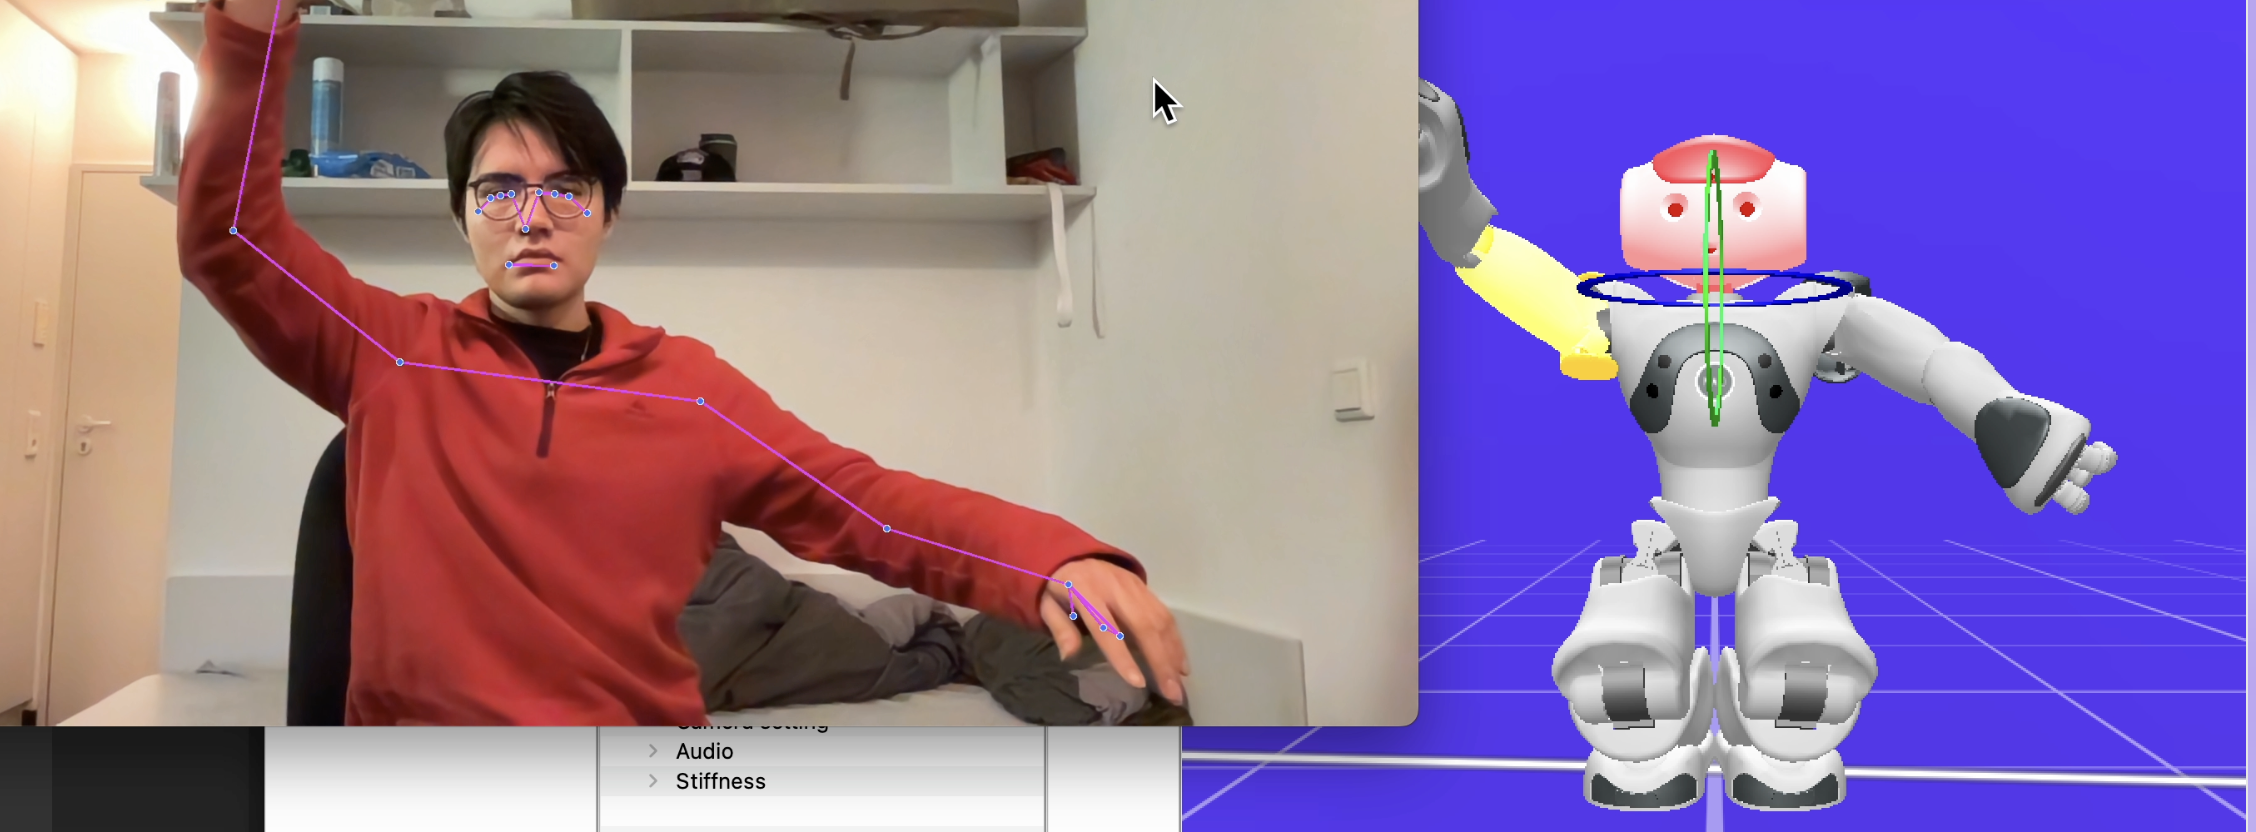
\includegraphics[width=0.48\textwidth]{images/RobotSimulation.png}}
\caption{NAO robot in the Choreographe simulator.}
\label{RobotSimulation}
\end{figure}


\begin{figure}[htbp]
    \centerline{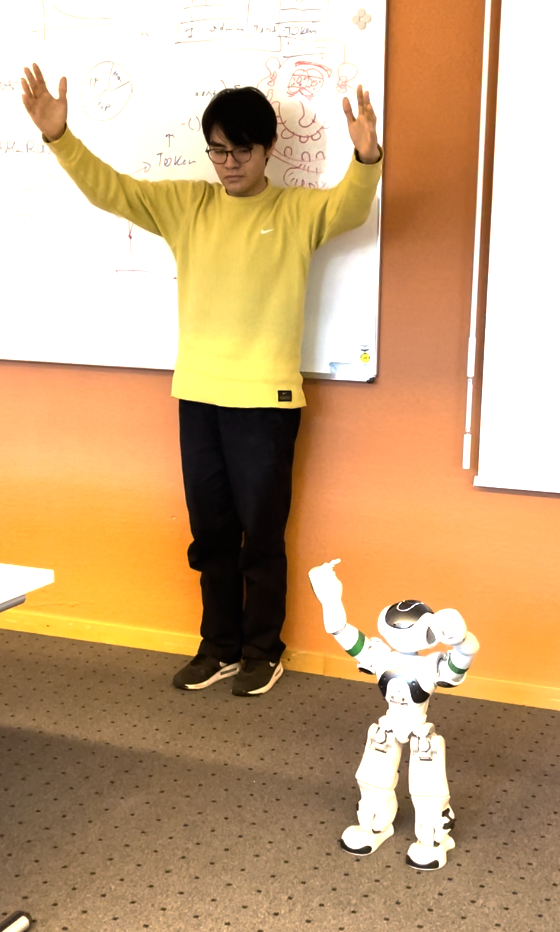
\includegraphics[width=0.4\textwidth]{images/RobotWorking.png}}
    \caption{NAO robot moving.}
    \label{RobotWorking}
    \end{figure}


We used a webcam and videos to see the angles that are being sent to the robot. To first initaite the application you have to run the server part, using a python 2.7 interpreter. 
This can be done using the following command, in which you have to specify the ip address of the robot as an argument:
\begin{verbatim}
    python2 server.py "ip_address"
\end{verbatim}
Then you have to run the client part, using a python 3.10 interpreter. 
If you want to send the landmarks using a webcam you can use the following command:
\begin{verbatim}
    python3 client.py 
\end{verbatim}
On the other hand, if you want to send the landmarks using a video you can use the following command:
\begin{verbatim}
    python3 client.py "path_to_video"
\end{verbatim}


Sometimes the robot falls and if this occurs the application might not work or would stop working, so we had to be careful about this, because sudden movements of the robot could make it fall. 
If the application stops working, there is no other option than to restart the application repeating the steps above.


% contrains of the experiments
% results of the experiments and description of data






\section{Conclusion and future work}
Even though the project is not finished, we think is a good start for just using computer vision to apply it in robotics.
\\
There is a lot of work to do, such as improving the calculation of the angles or use both inverse kinematics and programming the angles to move the robot.
\\
In order to use the legs of the robot is necessary to do further research, because we have to consider many other things such as the mass center of the robot, and take care that the movements are not too abrupt to make the robot fall.

% Acknowledgment
\section*{Acknowledgment}
We want to thank my proffesor, Dr. Christian Groth for helping us during the project and thank also to the Hof University of Applied Science for giving us the opportunity to work with the NAO robot, which was a great experience.


% Bibliography

% para citar \cite{b7}.
\begin{thebibliography}{00}

\bibitem{b1} NAOqi API, \textit{http://doc.aldebaran.com/2-5/naoqi/motion/index.html}
\bibitem{b2} Mediapipe Pose Landmarking\textit{https://developers.google.com/mediapipe
/solutions/vision/pose\_landmarker}
\bibitem{b3}I. Irigoyen, "Mimetización de movimiento por robot antropomorfo basado en imágenes de sensor de profundidad," Trabajo Fin de Grado, Facultad de Informática, Grado de Ingeniería Informática, Universidad del País Vasco, 2020.
\bibitem{b4} Nicholas Renotte - Robotics and AI, "AI Pose Estimation with Python and MediaPipe," YouTube, 2021. [Online]. Available: https://www.youtube.com/watch?v=06TE\_U21FK4&t=2109s&ab\_channel=
NicholasRenotte.


\end{thebibliography}

\end{document}
